\usetikzlibrary{shapes.geometric}

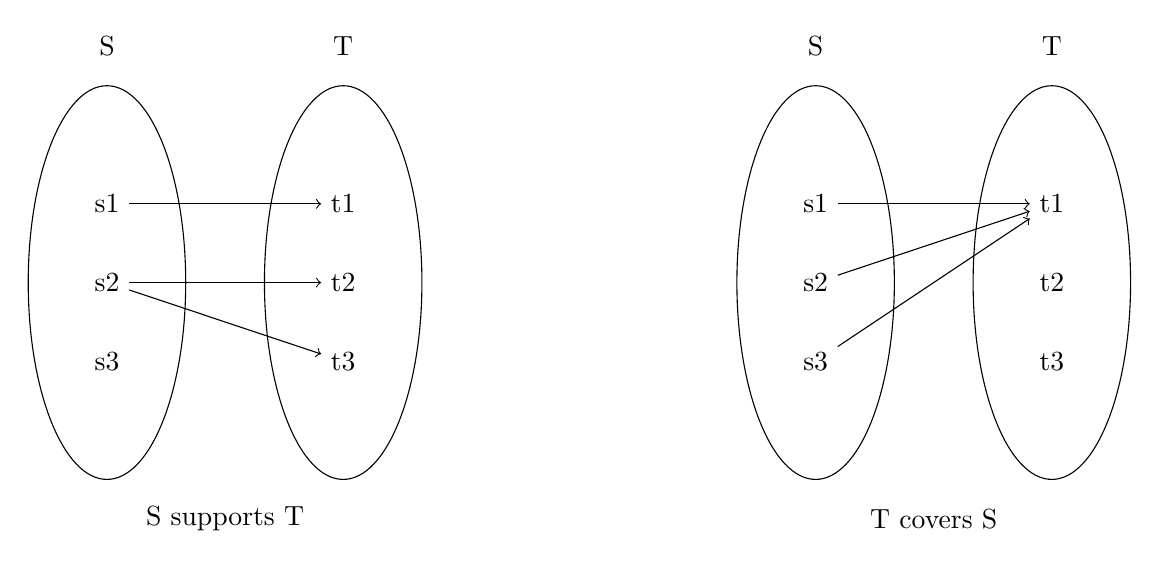
\begin{tikzpicture}


    \node[ellipse,
    draw = black,
    minimum width = 2cm, 
    minimum height = 5cm] (e) at (-6,0) {};

    \node[ellipse,
    draw = black,
    minimum width = 2cm, 
    minimum height = 5cm] (e) at (-3,0) {};

    \node[ellipse,
    draw = black,
    minimum width = 2cm, 
    minimum height = 5cm] (e) at (3,0) {};

    \node[ellipse,
    draw = black,
    minimum width = 2cm, 
    minimum height = 5cm] (e) at (6,0) {};


    \node[] (a1) at (-6,1) {s1};
    \node[] (a2) at (-6,0) {s2};
    \node[] (a3) at (-6,-1) {s3};

    \node[] (a1') at (-3,1) {t1};
    \node[] (a2') at (-3,0) {t2};
    \node[] (a3') at (-3,-1) {t3};

    \node[] (b1) at (6,1) {t1};
    \node[] (b2) at (6,0) {t2};
    \node[] (b3) at (6,-1) {t3};

    \node[] (b1') at (3,1) {s1};
    \node[] (b2') at (3,0) {s2};
    \node[] (b3') at (3,-1) {s3};

    \node[] (label) at (-4.5, -3) {S supports T};
    \node[] (label) at (4.5, -3) {T covers S};

    \node[] (label) at (-6, 3) {S};
    \node[] (label) at (-3, 3) {T};

    \node[] (label) at (3, 3) {S};
    \node[] (label) at (6, 3) {T};


      \draw[->] (a1) to (a1');
      \draw[->] (a2) to (a2');
      \draw[->] (a2) to (a3');

      \draw[->] (b1') to (b1);
      \draw[->] (b2') to (b1);
      \draw[->] (b3') to (b1);
  \end{tikzpicture}